\documentclass[12]{article}

\usepackage[margin=1in]{geometry}

\usepackage{tikz}
\usetikzlibrary{matrix,calc,shapes}
\tikzset{
	treenode/.style = {shape=rectangle, rounded corners,
		draw, anchor=center,
		text width=6em, align=center,
		top color=white, bottom color=blue!20,
		inner sep=1ex},
	decision/.style = {treenode, diamond, inner sep=0pt},
	root/.style     = {treenode, font=\Large,
		bottom color=red!30},
	env/.style      = {treenode, font=\ttfamily\normalsize},
	finish/.style   = {root, bottom color=green!40},
	dummy/.style    = {circle,draw}
}



\usepackage{xcolor,rotating,multirow} % for whatever reason, need to call xcolor before minted

\usepackage{minted} % and minted definitely has to precede gb4e
\newmintinline{python}{showspaces}

\usepackage{gb4e}

\usepackage[round]{natbib}
\usepackage{tipa,setspace}








\doublespacing

\title{Manual: The Gradient Lexicon and Phonology Learner}
\author{Claire Moore-Cantwell}
\date{\today}


\begin{document}

\maketitle

\section{Quick Start}

\section{Details of Theories Implemented}
	\subsection{Preliminaries}
		\subsubsection{Theories of \textsc{Eval}}

		\subsubsection{Perceptron Learning}
		
		- basic input to get frequency matching
			- within-word variation
			- across-word variation
		
		
		Getting the observed output candidate:
		
		- threshold vs. sampling
		
		
	\subsection{UseListed}
		UseListed is a theory that many researchers implicitly or explicitly use as a default approach to exceptionality in phonology, but as far as I know no learning model has been developed.  The theory can easily be summarized as "We memorize exceptions."
		
		This theory assumes two things:
		\begin{enumerate}
			\item We memorize morphologically complex words, at least sometimes
			\item We can therefore produce morphologically complex forms in two ways:
			\begin{itemize}
				\item {\bf Composed} forms are created by accessing multiple morphemes and realizing them together according to the morphological and phonological grammar
				\item {\bf Listed} forms are accessed whole, and realized according to their lexical entry and the phonological grammar
			\end{itemize}
		\end{enumerate}
	
		A couple of examples: 
							
		In Tagalog, morphemes often undergo 'nasal substitution' in which the final nasal of a prefix coalesces with the initial consonant of the root, forming a single sound.
		
		
		\begin{exe}
			\ex
				\begin{xlist}
					\ex \gll {\bf d}in\'i\textscriptg  \hspace{3ex} /pa{\bf \textipa{N}}+{\bf d}in\'i\textscriptg/ \hspace{8ex} $\rightarrow$ pa{\bf n}-{\bf d}in\'i\textscriptg   \hspace{7ex} \textsc{Assimilation}\\
					{\it audible} {} {} {} {\it sense of hearing}\\
					\ex \gll {\bf d}al\'a\textipa{N}in \hspace{0.1ex} /i+pa{\bf \textipa{N}}+{\bf d}al\'a\textipa{N}in+in/  $\rightarrow$ \textglotstop i-pa-{\bf n}al\'a\textipa{N}in-in \hspace{0.5ex} \textsc{Substitution}\\
					{\it prayer} {} {} {} {\it to pray}\\
				\end{xlist}
			
		\end{exe}
	
		These examples come from \citet{zuraw10}.  In (1a), the underlying velar nasal assimilates in place to the following stop, but in (1b), the two sounds have completely merged, leaving an [n] with the nasality of the [\textipa{N}] and the place of the [d].
		
		As the example suggests, the phonological shape of the individual words cannot completely predict whether the nasal will substitute or just assimilate.  There are lexical trends, but no categorical rules.  Importantly, individual words do not vary, the variation is entirely from word to word.
		
		A UseListed approach to this pattern would say that both pa{\bf n}-{\bf d}in\'i\textscriptg\ and \textglotstop i-pa-{\bf n}al\'a\textipa{N}in-in are memorized as their own lexical entries.  When speakers want to say the meaning {\it `sense of hearing'}, or {\it `to pray'}, they access those meanings directly in their lexicon, and produce them according to the idiosyncratic phonological form that is listed - one with substitution, and one without.
		
		\hspace{2ex}
		
		A second example: 
		
		English comparatives come in two forms, the `periphrastic', using {\it more}, and the `morphological', using {\it -er}.  Both are available for most adjectives: {\it fouler} and {\it more foul} are about equally attested in a corpus, for example.  However, higher-frequency adjectives exhibit idiosyncratic preferences \citet{smithmoorecantwell17}.
		
		\begin{exe}
			\ex \begin{xlist}
				\ex simpler (96\%) $\gg$ more simple (4\%)
				\ex more stable (98\%) $\gg$ stabler (2\%)
			\end{xlist}
		\end{exe}
		
		While a variety of phonological factors condition the choice between these two versions of the comparative, {\it simple} and {\it stable} are similar on all relevant dimensions\footnote{They are 2-syllable words with initial stress, ending in [l], and are about the same lexical frequency.}.  English speakers therefore must memorize that the meaning {\it simple + \textsc{Comparative}} is pronounced with {\it -er}, while {\it stable + \textsc{Comparative}} is pronounced with {\it more}.
		
		Unlike in the case of Tagalog nasal substitution, many individual words do vary, and low-frequency words seem to follow the predictions of a probabilistic grammar.  Even extreme cases like those in (2) still exhibit the minority form occasionally.  One was to imagine what is happening here is that speakers have memorized the majority form for both words, but every so often they fail to use that memorized form and compose the comparative on the fly instead.
		
		\hspace{2ex}
		
		
		If we have both a {\bf Composed} form and a {\bf Listed} form available, there are many different ways we could decide between them.  GLaPL can learn using any of these.
		
		\begin{itemize}
			\item[] {\bf Option 1:} Always use the listed form, if available.  OR use the listed form with some static probability
			\item[] {\bf Option 2:} Do whatever is easier.  If it is easy to find the listed form, use it, but if it is easier to compose, use the composed form.
			\item[] {\bf Option 3:} Directly compare the Composed and Listed derivations in the same tableau.
		\end{itemize}

		To do {\bf Option 1}, set \texttt{p\_useListed} to 1 or less.  That will be the probability that a \textsc{Predict} step will use the listed form, if available.
		
		To do {\bf Option 2}, set \texttt{p\_useListed} to 2. There are many possible ways to implement `easier' here, but for now the implementation is based on lexical frequency.  The probability that the listed form will be chosen is related to both the frequency of the listed form itself and the frequency of the lowest-frequency morpheme in the composed form.  
		
		\[
		P(listed) = \frac{freq_{listed}}{freq_{listed} + min(\{freq_{composed1}, freq_{composed2}\ldots freq_{composedx}\})}
		\]
		
		Hay 2003, Forster and Chambers 1973, Whaley 1987 % refs from Liu 2022?
		%Let's take the comparatives as an example.  Some adjectives occur often in comparative form (tall, large) while others occur in the comparative only rarely (fresh, cozy)

		Note: A lexeme name cannot start with a digit.  Can have a digit inside tho.

	\subsection{Lexically Indexed Constraints}
		
		In order to do actual locality restrictions, you need to write your constraint functions to return the indices of the violation(s).  make it a list: [[v1,v2...vn],[(start1,end1),(start2,end2)...(startn, endn)]]
		
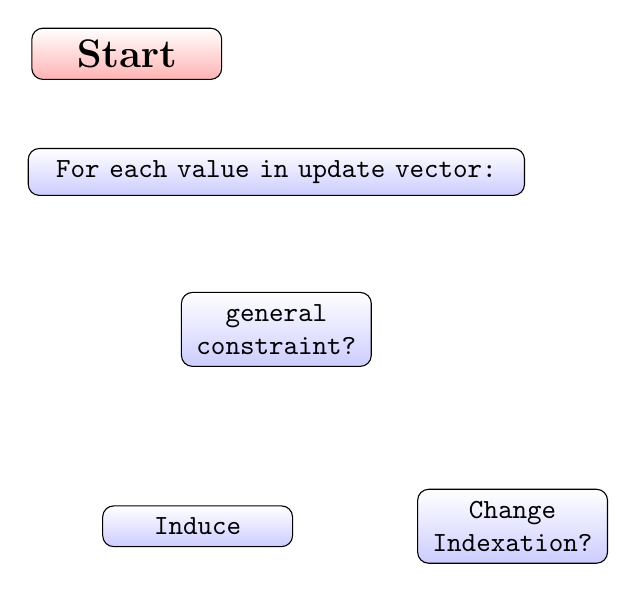
\begin{tikzpicture}[node distance = 2cm]
	\node [root, fill=blue!20] at (-.9,0) (start) {\textbf{Start}};
	\node [env, text width = 6cm] at (1,-1.5) (foreachupdate) {For each value in update vector:};
	\node [env, below of = foreachupdate] (generalC) {general constraint?};
	\node [env] at (0,-6)  (induce) {Induce};	
	\node [env] at (4,-6) (changeI) {Change Indexation?};	
\end{tikzpicture}

		
	\subsection{UR-constraints}

	\subsection{Representational Strength Theory}

	\subsection{Gradient Symbolic Representations}


\section{Supplementary details}
	\subsection{How Tableaux are constructed}
	Tableaux are constructed in real time during learning. At each learning iteration, a tableau is constructed for that input-output pair.  Here is a breakdown of how the \texttt{Grammar.makeTableau()} function operates.
	
	\texttt{Grammar.makeTableau()}'s first argument is a {\bf datum}, which is an entry in \texttt{Grammar.trainingData.learnData}, a list.
	
	\begin{exe}
		\ex {\bf datum:}  [[\texttt{lexeme\textsubscript{1}}, \texttt{lexeme\textsubscript{2}}, \ldots \texttt{lexeme\textsubscript{n}}], surface string, input]
	\end{exe}

	The surface string and input (also a string) both come directly from the input file.  The surface string comes either from your `candidate' column, or from your `surface' column, if you have one.  The input string comes from your `input' column.
	
	{\bf datum}'s first entry is a list of \texttt{lexeme} objects involved in this learning datum.  Note that if you are using UseListed, these won't always be the actual lexemes used to generate the tableau - the function may try to use the listed form instead.
	
	The first step in creating a tableau is to generate faithful candidates from the input lexemes.  In most cases, this will be a single faithful candidate, but not always.  The inner function \texttt{lexemesToFaithCands()} accomplishes this.
	
	In order to directly test \texttt{lexemesToFaithCands()} behaviour on a list of lexemes, run \texttt{makeTableau()} with the option \texttt{textFcs=True}.
	
	\begin{minted}[linenos,autogobble,bgcolor=lightgray]{python}
		import learner as l
		g = l.Grammar("lexemes_sampler.txt", l.Features("features.txt"))
		g.makeTableau([lexemes],testFcs=True)
		g.makeTableau([l.exlex_petit(),l.exlex_ami()],rich=True,testFcs=True)
	\end{minted}
	
	You can find ``lexemes\_sampler.txt" in the manual\_examples folder
	
	
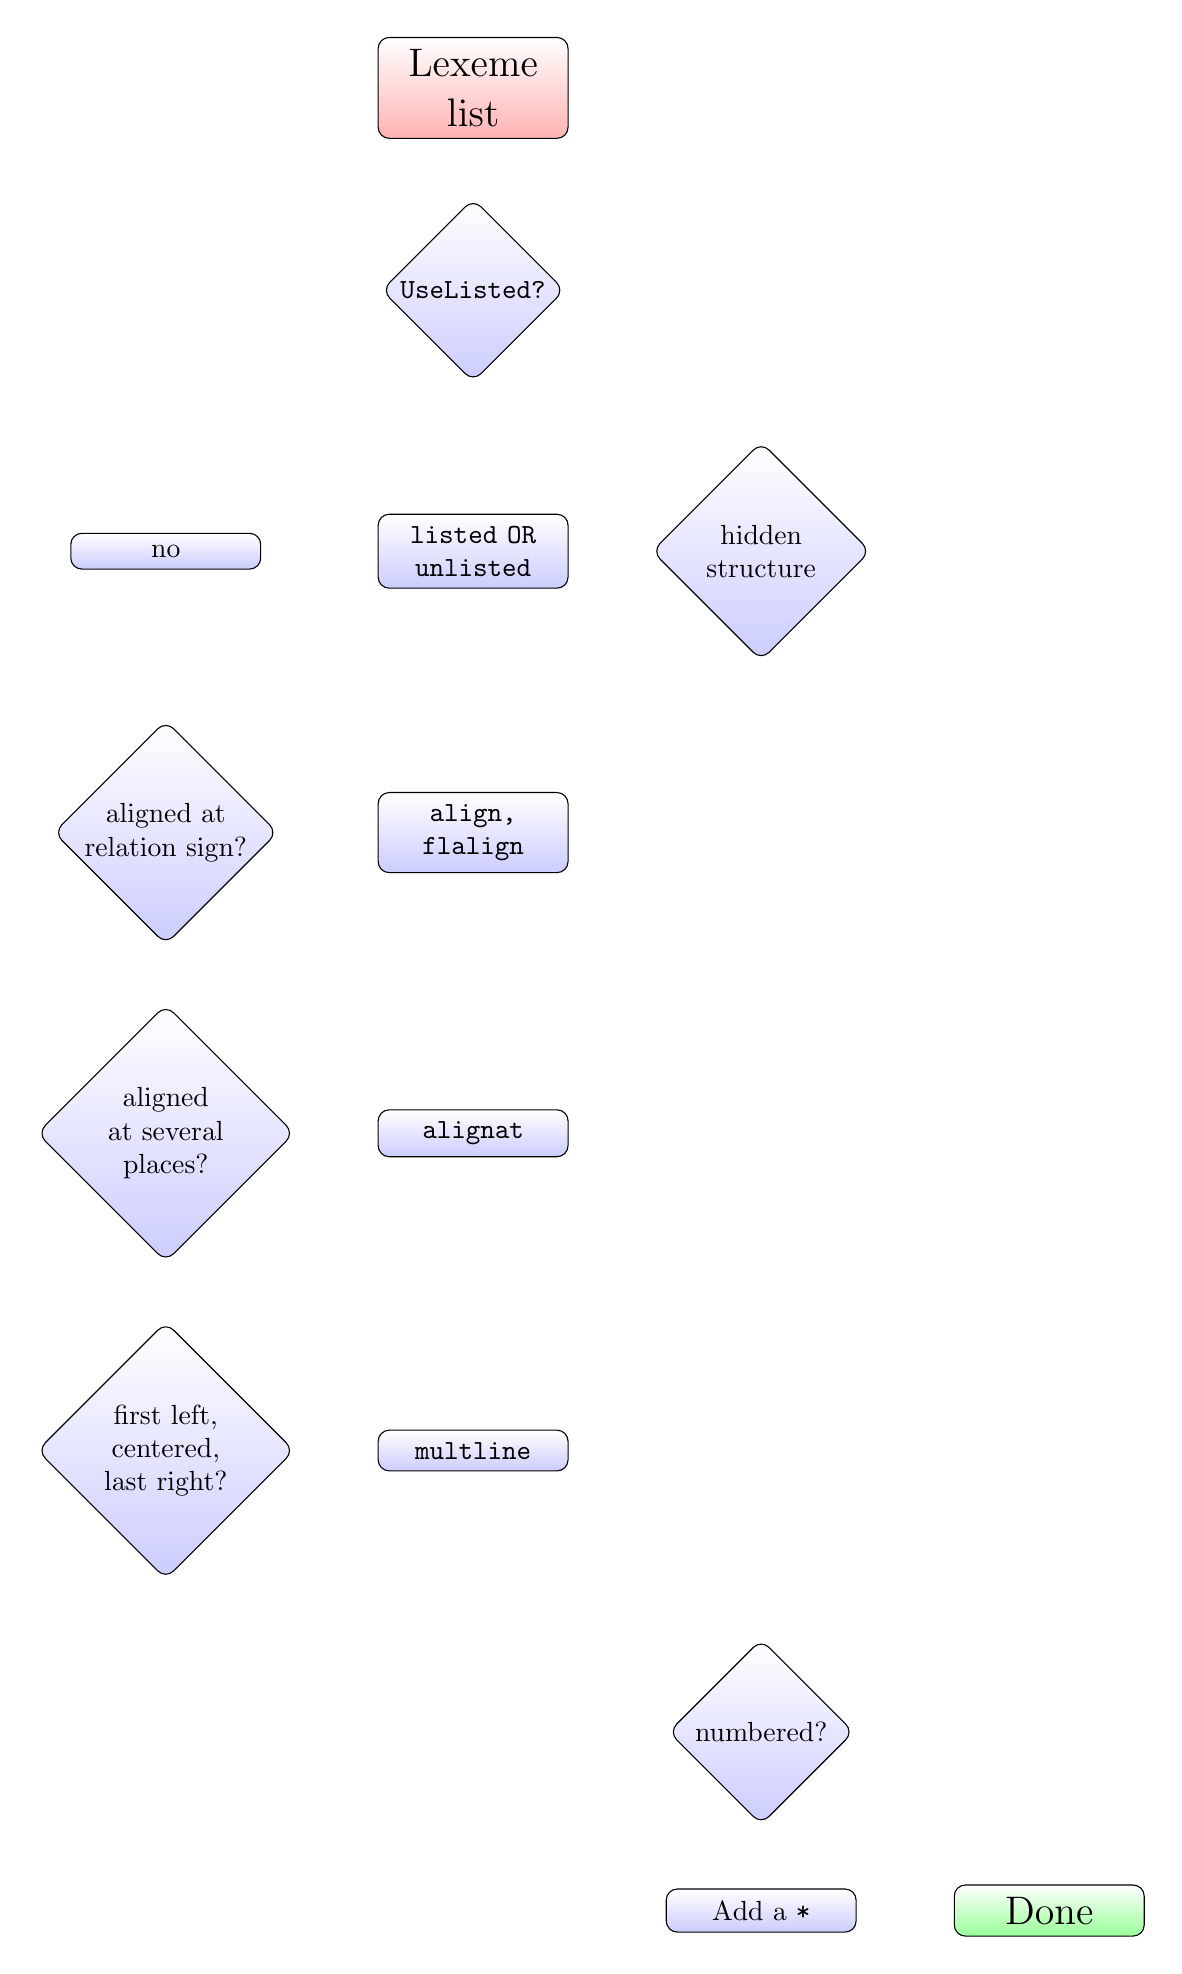
\begin{tikzpicture}
	\matrix (chart)
	[
	matrix of nodes,
	column sep      = 3em,
	row sep         = 5ex,
	column 1/.style = {nodes={decision}},
	column 2/.style = {nodes={env}},
	column 3/.style = {nodes={decision}}
	]
    {
	&	|[root]| Lexeme list       &                 \\
	&|[decision]| UseListed?             &      \\
	|[treenode]|no & |[treenode]|listed OR unlisted    & hidden structure          \\
	aligned at relation sign?  & align, flalign  \\
	aligned at several places? & alignat         \\
	first left, centered,
	last right?              & multline        \\
	& & |[decision]| numbered? \\
	& & |[treenode]| Add a \texttt{*}
	& |[finish]| Done \\
};


\end{tikzpicture}
	
	
	
	
	
	
	
	
	\subsection{Dealing with hidden Structure}
	
	Hidden structure problems can arise in any theory you are using, but UR-constraint models, UseListed with the \textsc{UseListed} constraint, and GSR models with segment blending all require hidden structure to operate.  GLaPL follows the principles of Jarosz (2013)'s Expectation-Maximization algorithm ot learn hidden structure.  
	
	Let's look at an example using \textsc{UseListed}.  UR-constraints would function similarly. 
	
	  \begin{exe}
	  	\ex\label{useListedHiddenTab} Tableau for made-up multi-morphemic word, based on Pater et al, 2012.
	  	
	  	\begin{tabular}{llll|ccc|cc}
	  		
	  		  &          &  &                  &\textsc{*VTV} & \textsc{Ident-Voice} & \textsc{UseListed} &   &  \\
	  		  &          & &       weights:    &  1  &  2          &   1       & H & p \\  
	  		  \hline 
	  		  &&&&&&&\\

\multirow{2}{*}{\rotatebox{90}{\parbox{9ex}{Composed}}}	  		&a.& /mot/+/a/& $\rightarrow$ mota &  1  &  0          &   1    	  & -2&0.11 \\
	  		&b.& /mot/+/a/& $\rightarrow$ moda &  0  &  1          &   1       & -3&0.04\\
\multirow{2}{*}{\rotatebox{90}{\parbox{9ex}{Listed}}}		  	&	c.& /moda/   & $\rightarrow$ mota &  1  &  1          &   0       & -3&0.04\\
	  		&d.& /moda/   & $\rightarrow$ moda &  0  &  0          &   0       & 0 &0.81\\
	  	
	  	\end{tabular}
	  
	  \end{exe}
	  
	  
	  In (\ref{useListedHiddenTab}), candidates a. and b. come from a UR that concatenates two morphemes' URs, while c. and d. come from a single UR, the listed lexical item that combines the meanings of \textsc{Mot} and \textsc{-a}.  In this example, the combined form of the two has a voiced stop instead of a voiceless one.  Candidates a. and c. have different violation profiles: The [d] is a faithfulness violation for the composed form, but the [t] is a faithfulness violation in the listed form.  \textsc{UseListed} also assigns violations differently.  The same is true for candidates b. and d.  Each of these pairs sounds identical, however.  Suppose the correct form is [moda].  If on a given learning iteration, we sample either candidate b. or candidate d., this prediction would count as correct.  This would not cause any problem, the learner simply would not update.  However, if candidate a. or c. were sampled, this would count as an error, and we would need to update constraint weights.
	  
	  Suppose we sampled candidate a.  That candidate would be the {\bf predicted} candidate for perceptron update, but in order to update we need to compare it to an {\bf observed} candidate.  b. and d. both correspond to the actual observed output, so either one could plausibly be used as the {\bf observed} candidate.  How do we choose between them?
	  
	  One option, of course, is simply to designate one of them correct.  Perhaps we could decide that we want the learner to always learn the Composed form, so a. is always the {\bf observed} candidate.  However, in this case we are determining the hidden structure in advance instead of allowing the learner to choose the most optimal hidden structure.  In the \textsc{UseListed} case, we would be forcing the learner not to use listed forms.  Note: if you do want to run a simulation like this with GLaPL, you can just turn lexical listing off to achieve the same effect.
	  
	  We could also sample at random between the two correct candidates.  The trouble with this approach is that it fails to take into account what the learner already knows, forcing it to essentially reconsider hypotheses that it has already rejected.  Much better would be to take into account the weights the learner has already arrived at, which predict that d. should be much more likely than b.
	  
	  To do this, we create a mini-tableau considering only candidates whose surface form corresponds to the observed correct output form in our data.
	  
	  \begin{exe}
	  	\ex\label{observedGrabber} To get the observed form, consider only candidates whose surface form corresponds to the correct output.
	  	
	  	\begin{tabular}{lll|ccc|cc}
	  		
	  		& &                  &\textsc{*VTV} & \textsc{Ident-Voice} & \textsc{UseListed} &   &  \\
	  		& &       weights:    &  1  &  2          &   1       & H & p \\  
	  		\hline 
	  		
	  		b.& /mot/+/a/& $\rightarrow$ moda &  0  &  1          &   1       & -3&0.05\\
	  		d.& /moda/   & $\rightarrow$ moda &  0  &  0          &   0       & 0 &0.95\\
	  		
	  	\end{tabular}
	  	
	  \end{exe}
  
  	In (\ref{observedGrabber}), candidate d. is vastly more likely to be sampled than b.  95\% of the time, we will use that one as the {\bf observed} candidate.
  	
  	To see why it is so important to sample according to the current state of the grammar, consider another type of hidden structure: foot structure in a stress system.
  	
  	\begin{exe}
  	\ex\label{stressHiddenStructureTab} Tableau for made-up multi-morphemic word, based on Pater et al, 2012.
  	
  	\begin{tabular}{ll|cccc|cc}
  		
  		 &                  &\textsc{Align-R} 	& \textsc{Align-L} 	& \textsc{Iamb}	& \textsc{Trochee} 	&     &   \\
  		 &       weights:   &		0.1			&		0.2			&		0.2		&		3			& H   & p \\  
  		\hline 
  		a. & (pat\'{a})ka 	&		1			&		0			&		0		&		1			& 3.1 & 0.03 \\
  		b. & pa(t\'{a}ka)   &		0			&		1			&		1		&		0			& 0.4 &	0.41 \\
  		c. & (p\'{a}ta)ka   &		1			&		0			&		1		&		0			& 0.1 &	0.55 \\
  		d. & pa(tak\'{a})	&		0			&		1			&		0		&		1			& 3.4 &	0.20 \\
  	\end{tabular}
  	
  \end{exe}	

	In (\ref{stressHiddenStructureTab}), candidates a. and b. have the same surface form: [pat\'{a}ka].  They differ only on whether that stress pattern is the result of a right-aligned trochee, or a left-aligned iamb.  Other words in the language would not have such an ambiguity.  A two-syllable word, /pata/, would either be stressed on the first syllable, (p\'ata), which could only be a trochee, or the second (pat\'a), which could only be an iamb (assuming two syllable feet).
	
	So, assuming that the relatively high weight on \textsc{Trochee} comes from learning on forms like this in the language, we want the learner to take this into account in choosing a foot structure for pat\'aka.  Suppose the learner predicted candidate c. to be the winner, and chose candidate a. as the {\bf observed} candidate.  The update would then look like this:
	
	\begin{exe}
		\ex\label{stressWrongUpdate} Update vector for (p\'ata)ka $>$ (pat\'a)ka.  (Learning rate 0.01)
		
		\begin{tabular}{ll|cccc}
  		 &                  &\textsc{Align-R} 	& \textsc{Align-L} 	& \textsc{Iamb}	& \textsc{Trochee} \\
  		 &  {\it weights:} 	&		0.1			&		0.2			&		0.2		&		3			\\
  		 \hline
{\bf predicted}	& (pat\'a)ka &		1			&		0			&		0		&		1			\\
{\bf observed}	& (p\'ata)ka &		1			&		0			&		1		&		0			\\
		\hline
		 & {\it new weights:}&		-			&		-			&		0.21	&		0.29		\\
		\end{tabular}
		
	\end{exe}
	

If this update happens, both \textsc{Trochee} and \textsc{Iamb} will move in the wrong direction.  Compare to the update that would happen if we chose candidate b. as the {\bf observed} form:
  	
  	
	\begin{exe}
	\ex\label{stressRightUpdate} Update vector for (p\'ata)ka $>$ pa(t\'aka).  (Learning rate 0.01)
	
	\begin{tabular}{ll|cccc}
		&                  &\textsc{Align-R} 	& \textsc{Align-L} 	& \textsc{Iamb}	& \textsc{Trochee} \\
		&  {\it weights:} 	&		0.1			&		0.2			&		0.2		&		3			\\
		\hline
{\bf predicted}	& pa(t\'aka) &		0			&		1			&		1		&		0			\\
{\bf observed}	& (p\'ata)ka &		1			&		0			&		1		&		0			\\
		\hline
& {\it new weights:} 		 &		0.11		&		0.19		&		- 		&		-			\\
	\end{tabular}
	
\end{exe}

In (\ref{stressRightUpdate}), \textsc{Align-R} goes up a little, \textsc{Align-L} goes down a little.  This update is preferable to the one in (\ref{stressWrongUpdate}), because it doesn't backtrack on what the learner has already figured out from other forms, and it {\it does} get information about the \textsc{Align} constraints from the error, learning that it should prefer right-alignment over left-alignment.  Two-syllable forms which would be informative about \textsc{Iamb} vs. \textsc{Trochee} would be uninformative about alignment.

In summary, if we chose the candidate already preferred by the grammar, candidate b., we will get an update that is more informative, and pushes the grammar in a direction compatible with previously encountered data.  For this reason, Jarosz (2013) recommends a procedure like that demonstrated in (\ref{observedGrabber}), and that is what is implemented in GLaPL.

One last thing to note is that hidden structure can arise in a lot of different ways.  We've looked at foot structure, and underlying form here, but most Gradient Symbolic Representation analyses will also have a hidden structure component.  Here's an example to illustrate:


\begin{exe}
	\ex\label{GSRhidden} Sample GSR tableau showing hidden structure.  Activity on t\textsubscript{a} is 0.7, and on t\textsubscript{b} is 0.2
	
	\begin{tabular}{l|ccccc|cc}
				& \textsc{Max} & \textsc{Dep} & \textsc{Uniformity} & \textsc{NoCoda} & \textsc{*Hiatus} & H & p \\
	/petit/\textsubscript{a} + /{t,z,n}ami/\textsubscript{b} & 2 & 2 & 3 & 5 & 5 & & \\
	a. petiami &0&0&0&0& 1 & -5 & 0.57 \\
	b. petit\textsubscript{a}ami & -0.7 & 0.8 &0&0&0& 0.1 &0.21 \\
	c. petit\textsubscript{b}ami & -0.2 & 0.3 &0&0&0& 0.1 &0.01 \\
	d. petit\textsubscript{a,b}ami &0& 0.1 & 1&0&0& 00 & 0.21 \\
	
	\end{tabular}
	
\end{exe}


	  
	\subsection{Simulating \textsc{Gen}}
	\subsection{Applying constraints}

\section{Input file details}

\subsection{The \texttt{config.gl} file}

\texttt{config.gl} is where you will set almost all the parameters for learning.  You can create multiple versions of this file to save different parameter settings, and you can name them whatever you want.  You just then need to call \pythoninline{learner.Grammar()} with the config file you want to use as an argument:

\begin{minted}[linenos,autogobble,bgcolor=lightgray]{python}
	g = l.Grammar("myURCsConfig.gl")
\end{minted}

If no config file is specified, the learner will look for a file called \texttt{config.gl} in the same directory your console is pointed to (most likely the directory where the learner is).

{\bf Structure of the config file:} 

\begin{enumerate}
	\item Each line is a parameter setting of the form \texttt{parameterName: value}
	\item Lines that begin with `\#' will be ignored
\end{enumerate}

Whitespace is ignored.

{\bf Parameters and their values:}

\begin{itemize}
	\item[\texttt{trainingData}] 
	A string, the name of your input file.  No default value.
	
	\item[\texttt{weights}] A list of numbers, separated by commas.  The weights you would like your constraints to have at the beginning of learning.
	
	If you write a single 0, all weights will be initialized to 0.
	
	\item[\texttt{featureSet}]
	
	A string, the filename of your features file.
	
	For many use cases, this file is irrelevant, but you still have to specify something.  I recommend to just use the sample `features.txt' file that came with this manual.
	
	\item[\texttt{addViolations}]
	
	\pythoninline{True} or \pythoninline{False}.  Make sure you spell them the way Python likes, capital first letter and the rest lower case.
	
	If \pythoninline{True}, violations will be added to your tableaux during learning using the constraint functions that your provide.
	
	\item[\texttt{constraints}]
	
	A string, the name of your constraints file.  It should be a Python file, ending in .py, but you should leave off the .py here.
	
	\item[\texttt{generateCandidates}]
	\pythoninline{True} or \pythoninline{False}.  Make sure you spell them the way Python likes, capital first letter and the rest lower case.
	
	If \pythoninline{True}, candidates will be generated for you, using the operations you defined in your constraint file.
	
	\item[\texttt{operations}]  	\pythoninline{True} or \pythoninline{False}.  Make sure you spell them the way Python likes, capital first letter and the rest lower case.
	
	If \pythoninline{True}, ...  COLLAPSE THESE
	
	\item[\texttt{learningRate}] Float, indicating how much constraint weights should change on update.  Default value is 0.01
	
	\item[\texttt{decayRate}] Float, indicating how much to decay an object at each timestep.
	
	This value will be used to decay PFCs if you are using them, UR-constraints if you use them and decay them, Lexically-indexed constraints if you use them and decay them, etc.
	
	Default value is 0.0001
	
	\item[\texttt{threshold}] A float between 0 and 1, indicating how much observed probability a candidate must have to count as correct.
	
	{\bf Example:} Suppose candidates A, B, C with observed output probabilities of 0.6, 0.38, and 0.02, respectively.  If \texttt{threshold} is set to 0.1, then a predicted value of A or B would count as correct, but not C.
	
	If \texttt{threshold} is set to 1, an observed output will be sampled.  So, in the above example the observed output would be A 60\% of the time, B 38\% of the time, and C 2\% of the time.
	
	Note that it doesn't make sense to set \texttt{threshold} to 0, since this will result in no errors, and therefore no learning.
	
	\item[\texttt{noisy}]  String, ``yes" or ``no".
	
	If ``yes", learning will print out lots of updates to the console as it goes.
	
	\item[\texttt{useListedType}] String, 4 options:
	
	``hidden\_structure"  If chosen, the constraint \textsc{UseListed} will be added to the grammar, and tableaux will be constructed with listed and composed forms competing.
	
	``sample\_using\_frequency"  If chosen, either the listed form or the composed form will be chosen, sampled according to the relative frequency of the listed form and the {\it least frequent} morpheme in the composed form (usually the root if it's a root plus affixes)
	
	``sample\_flat\_rate"  If chosen, the listed form (if available) will be chosen at a flat rate, specified by you in the next parameter.
	
	``none"  No lexical listing will be used in learning.  (No new lexemes created)
	
	\item[\texttt{useListedRate}] Float, between 0 and 1.  Only used if you chose ``sample\_flat\_rate" above.  The chance that the listed form will be used, if available.
	
	Defaults to 1, always use the listed form if you can.
	
	\item[\texttt{flip}]  \pythoninline{True} or \pythoninline{False}.  Make sure you spell them the way Python likes, capital first letter and the rest lower case.
	
	Only relevant when inputs exhibit within-item variation in your data.  
	
	{\bf Example:} Suppose you have an input ``\textsc{Cat+Pl}", with two observed outputs, [moda] (30\%) and [mota] (70\%).  If \texttt{flip} is \pythoninline{True}, then the lexical entry for the listed form ``\textsc{Cat+Pl}" will be re-listed each time an error is made.  Its value will keep ``flipping" back and forth between /moda/ and /mota/.
	
	\item[\texttt{simpleListing}]\pythoninline{True} or \pythoninline{False}.  Make sure you spell them the way Python likes, capital first letter and the rest lower case.
	
	Only relevant when inputs exhibit within-item variation in your data.  
	
	If \pythoninline{True}, then a listed lexeme will only be created once, and never changed.  With the example from \texttt{flip} above, if [moda] happens to be sampled first, then the UR for ``\textsc{Cat+Pl}" will be encoded as /moda/.  If [mota] happens to be sampled first, then it will be encoded as /mota/.
	
	\item[\texttt{pToList}]  Float, between 0 and 1.  If lexical listing is enabled (\texttt{useListedType} is not ``none"), this is the probability that a complex form will be listed on error.  Defaults to 0.75
	
	\item[\texttt{nLexCs}] 0, any positive integer, or the string ``inf".  
	
	If not 0, lexically indexed constraints will be learned.
	
	If set to a positive integer, that integer is the maximum number of copies of each constraint that can be learned.
	
	If set to ``inf", there is no maximum number of copies.
	
	\item[\texttt{pChangeIndexation}] Float between 0 or 1.  The probability that on error, a lexical item will switch which copy of a constraint it is indexed to in order to improve performance.
	
	\item[\texttt{lexCStartW}] Float greater than 0.  The starting weight of any newly-induced lexically indexed constraints.
	
	\item[\texttt{PFC\_type}] String, 3 options:
	
	``full" PFCs will be induced based on generated candidates.
	
	``partial" PFCs will be induced based on given candidates.  They will not use features, but will simply prefer a specific candidate over all the others.  Refer to the Representational Strength Theory section to see how to set up your input file so this makes sense.
	
	``none" No PFCs will be induced.
	
	\item[\texttt{PFC\_lrate}]  Positive float.  The learning rate for PFCs - how much their weight will change on error.

	\item[\texttt{PFC\_startW}]	Float greater than 0.  The starting weight of any new PFC induced.

	\item[\texttt{activityUpdateRate}]  Positive float.  If using GSRs, the amount by which a segment's activity value will be updated on error.
	
\end{itemize}




\section{Classes and Methods}

\section{Files that should come with this manual}
features.txt, a sample features file for MAE

config.gl with default values

\end{document}
